% Planteamiento del Problema

\chapter{Metodología} % Chapter title

\label{ch:metodologia} % For referencing the chapter elsewhere, use \autoref{ch:introduction} 
\section{Actividades a realizar}

\subsection{1er Objetivo específico}
\subsubsection{Definición}
Definir un modelo general de evaluación de costos para el análisis de los servicios en el \acrshort{CC} usando información recuperable y relevante de la Web de sus proveedores.
\subsubsection{Actividades}
\begin{enumerate}
    \item Investigar acerca de las los modelos de precios en los \acrshortpl{CCSP}.
    \item Comparar los criterios de cobro entre cada \acrshort{CCSP}.
    \item Identificar las variables principales que usan los \acrshortpl{CCSP} para el cobro de los servicios.
    \item Efectuar pruebas de escritorio del modelo para 5 \acrshortpl{CCSP}.
\end{enumerate}
\subsubsection{Resultado esperado}
Ecuaciones del modelo listas para implementación

\subsection{2do Objetivo específico}
\subsubsection{Definición}
Diseñar e implementar un prototipo basado en microservicios que recopile periodicamente y almacene las tarifas de los principales \acrshortpl{CCSP}.
\subsubsection{Actividades}
\begin{enumerate}
    \item Diseñar el modelo de datos para almacenar la información de costos.
    \item Diseñar un microservicio que use técnicas de \emph{Crawling} y \emph{Scraping} para recuperar datos de precios de los \acrshortpl{CCSP}.
    \item Implementar el modelo de evaluación de costos usando un microservicio.
    \item Diseñar una configuración de microservicios en \gls{Docker Compose}.
    \item Desplegar la configuración de microservicios en \gls{Docker Compose}.
\end{enumerate}
\subsubsection{Resultado esperado}
Web service funcional que recopile y almacene información de costos de los \acrshortpl{CCSP}.

\subsection{3er Objetivo específico}
\subsubsection{Definición}
Diseñar e implementar un prototipo de aplicación web basada en microservicios para acceder a la información de costos de los proveedores y administrar los recursos de un usuario usando tecnologías agnósticas del proveedor.
\subsubsection{Actividades}
\begin{enumerate}
    \item Diseñar el modelo de datos para almacenar la información de la aplicación.
    \item Diseñar un microservicio para la administración básica de recursos sobre \acrshort{AWS} usando \gls{LibCloud}.
    \item Diseñar a partir de un microservicio una aplicación web usando \emph{NodeJS} con \emph{ReactJS} para proveer una interfaz de usuario.
    \item Diseñar una configuración de microservicios en \gls{Docker Compose}.
    \item Desplegar la configuración de microservicios en \gls{Docker Compose}.
\end{enumerate}
\subsubsection{Resultado esperado}
Prototipo de aplicación web para administrar recursos de tipo \emph{Compute}, \emph{Storage} y \emph{Container} sobre \acrshort{AWS} y obtener información de costos de los principales \acrshortpl{CCSP}.

\newpage
\section{Cronograma de Actividades}
A continuación se adjunta información referente al las actividades a desarrollar de la propuesta.
\begin{center}
    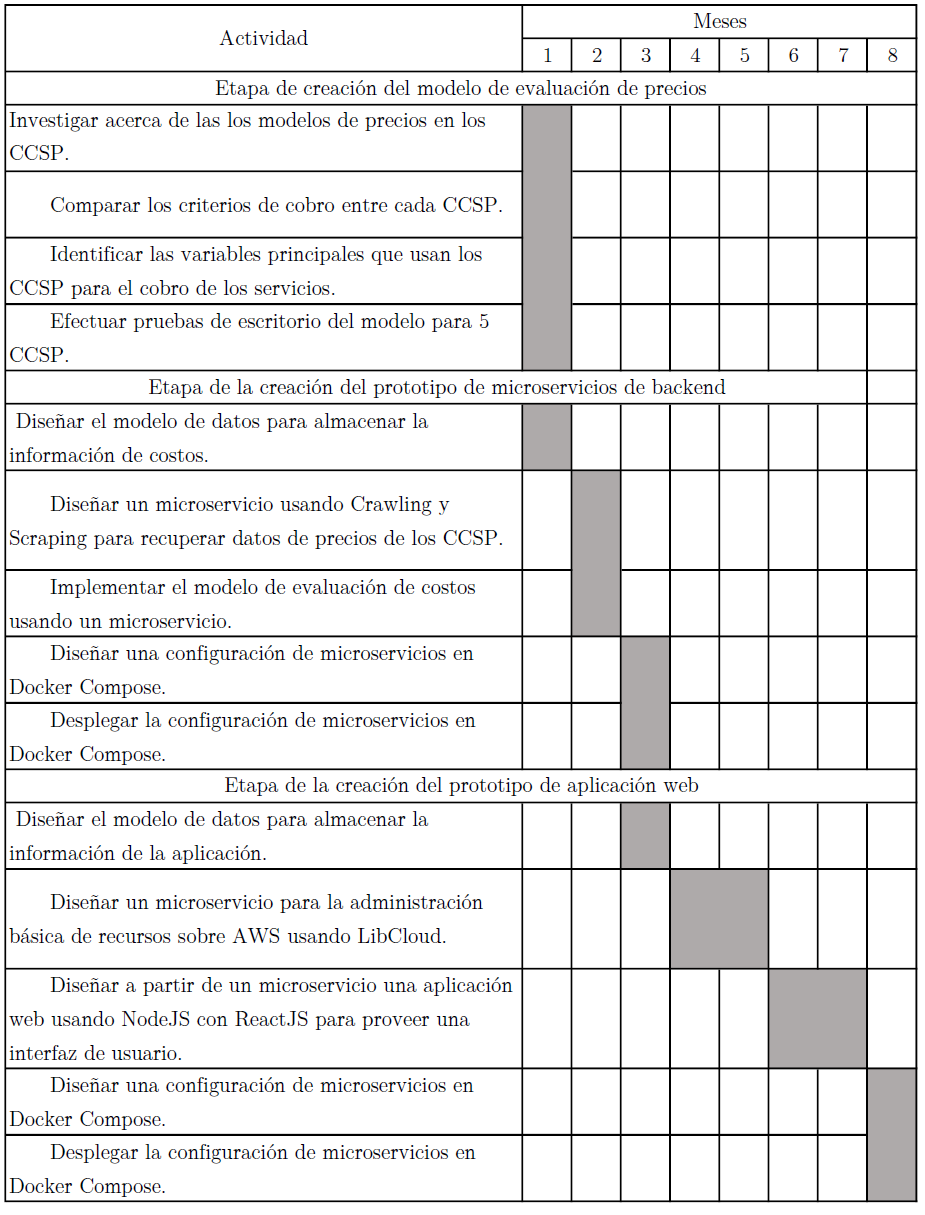
\includegraphics[width=\textwidth]{gfx/actividades3.png}
\end{center}

%----------------------------------------------------------------------------------------
